\section{Results}
\label{sec:results}

\subsection{App Pipeline}

The application will be stored on our GitHub repo. We have a transformer folder that includes all the transformer architecture and data directories for training and testing. The demo.py inside the transformer folder is the application we wanted to demo. It incorporates mediapipe, and when the user uses feed mode, the drawing canvas will be fed into the transformer to output \LaTeX\ code in the terminal. 

To use the demo, please run demo.sh script in our GitHub, which will create a virtual environment for the user, download all the packages in requirements.txt, and run demo.py in the transformer directory to start the application. Then follow the GitHub instruction or Section \ref{sec:drawingmodes} for enabling different MediaPipe modes. The current iteration of the application does not work on M1 Macs.

The application works as follows: the program first loads the transformer model checkpoint in the root directory. Then air drawing function is run that processes each frame of the camera video in real-time to analyze the user's hand. When the user enables feed mode, the drawing canvas will be saved as passed to the checkpoint model for \LaTeX\ conversion. 

\subsection{App Performance}
The application overall performs well. Figure~\ref{fig:mpmc} shows one of the results we got and that the transformer correctly convert our drawing of $e=mc^2$. 

There are some drawbacks, of course. For example, the whole hand has to be in the camera for MediaPipe to accurately identify the index fingertip. Furthermore, since MediaPipe constantly detects hands in each frame, there is no easy way to detect "pen up" operation. To counter this, the program enables drawing mode when the only finger raised is the right-hand index finger. Lifting the middle finger along with the index finger on the right hand can can pause drawing. This is slightly inconvenient for the user but is the only feasible solution we can come up with. 

One inconvenience of this application is that the user has to point the right index finger upward to enable drawing. This is because our implementation enables drawing when landmark 8 is higher than landmark 6 in Figure~\ref{fig:mplm}. Therefore, the user can not tilt his  hand to the point that makes landmark 8 less than landmark 6 when this index finger is raised. 


\begin{figure*}[h!]
    \centering
    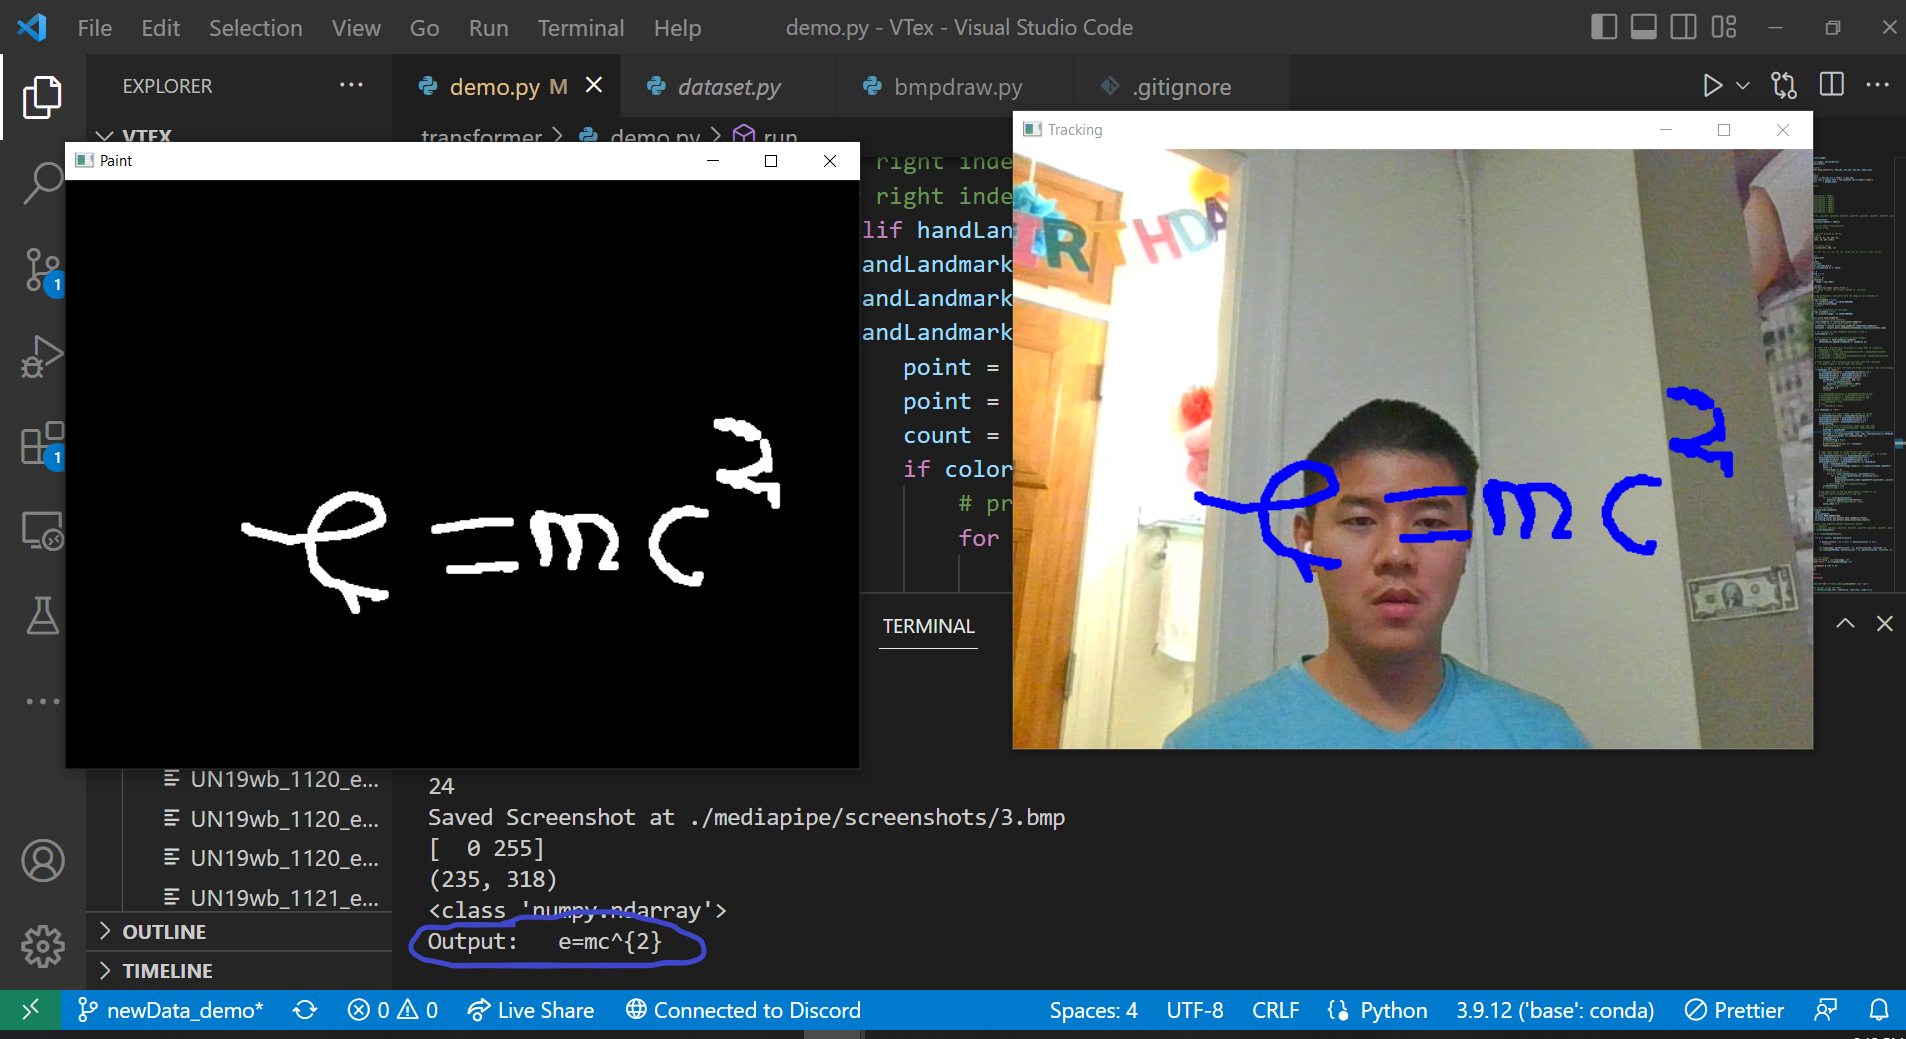
\includegraphics[width=15cm, height=7cm]{images/mc.png}
    \cprotect\caption{Example showing the correct \LaTeX\ conversion of our airdrawing of Einstein's famous equation. The program outputted \verb|e=mc^{2}|}
    \label{fig:mpmc}
\end{figure*}


\subsection{Neural Network Results}
\subsubsection{Training}
As mentioned in Section \ref{sec:datacollection}, the model is trained on the CROHME training dataset and validated on the CROHME 2014 test set. Figure \ref{fig:epoch1} shows the training progress of the transformer on two NVIDIA GeForce GTX 1070 GPUs using a batch size of 8. The red lines depict the validation loss, while the green lines depict the training loss. The training shows a significant improvement in both the training and validation loss until approximate epoch 20, when the training loss levels out and no longer decreases, and the validation loss becomes very noisy. Training is stopped after 500 epochs when it becomes clear that the total loss will no longer improve significantly. 

While the large fluctuations in validation loss is concerning, it was disregarded due to the loss's overall downward trend. Nonetheless, there are several possible reasons for this variance, including large learning rates, small batch sizes, and model complexity. We suspect that in this case, the variance is caused by a small validation set (986 vs. 8836 in the training set). If so, this can be easily remedied by transferring some data from the training set to the validation set. Alternatively, the overall training set can be dramatically increased by means of transfer learning, perhaps with the aforementioned {\tt IM2LATEX-100K} dataset \cite{im2latex}. Furthermore, while not implemented, an ensemble approach can aggregate the best performing epochs to reduce inconsistencies caused by the variance.

\begin{figure}[h!]
    \centering
    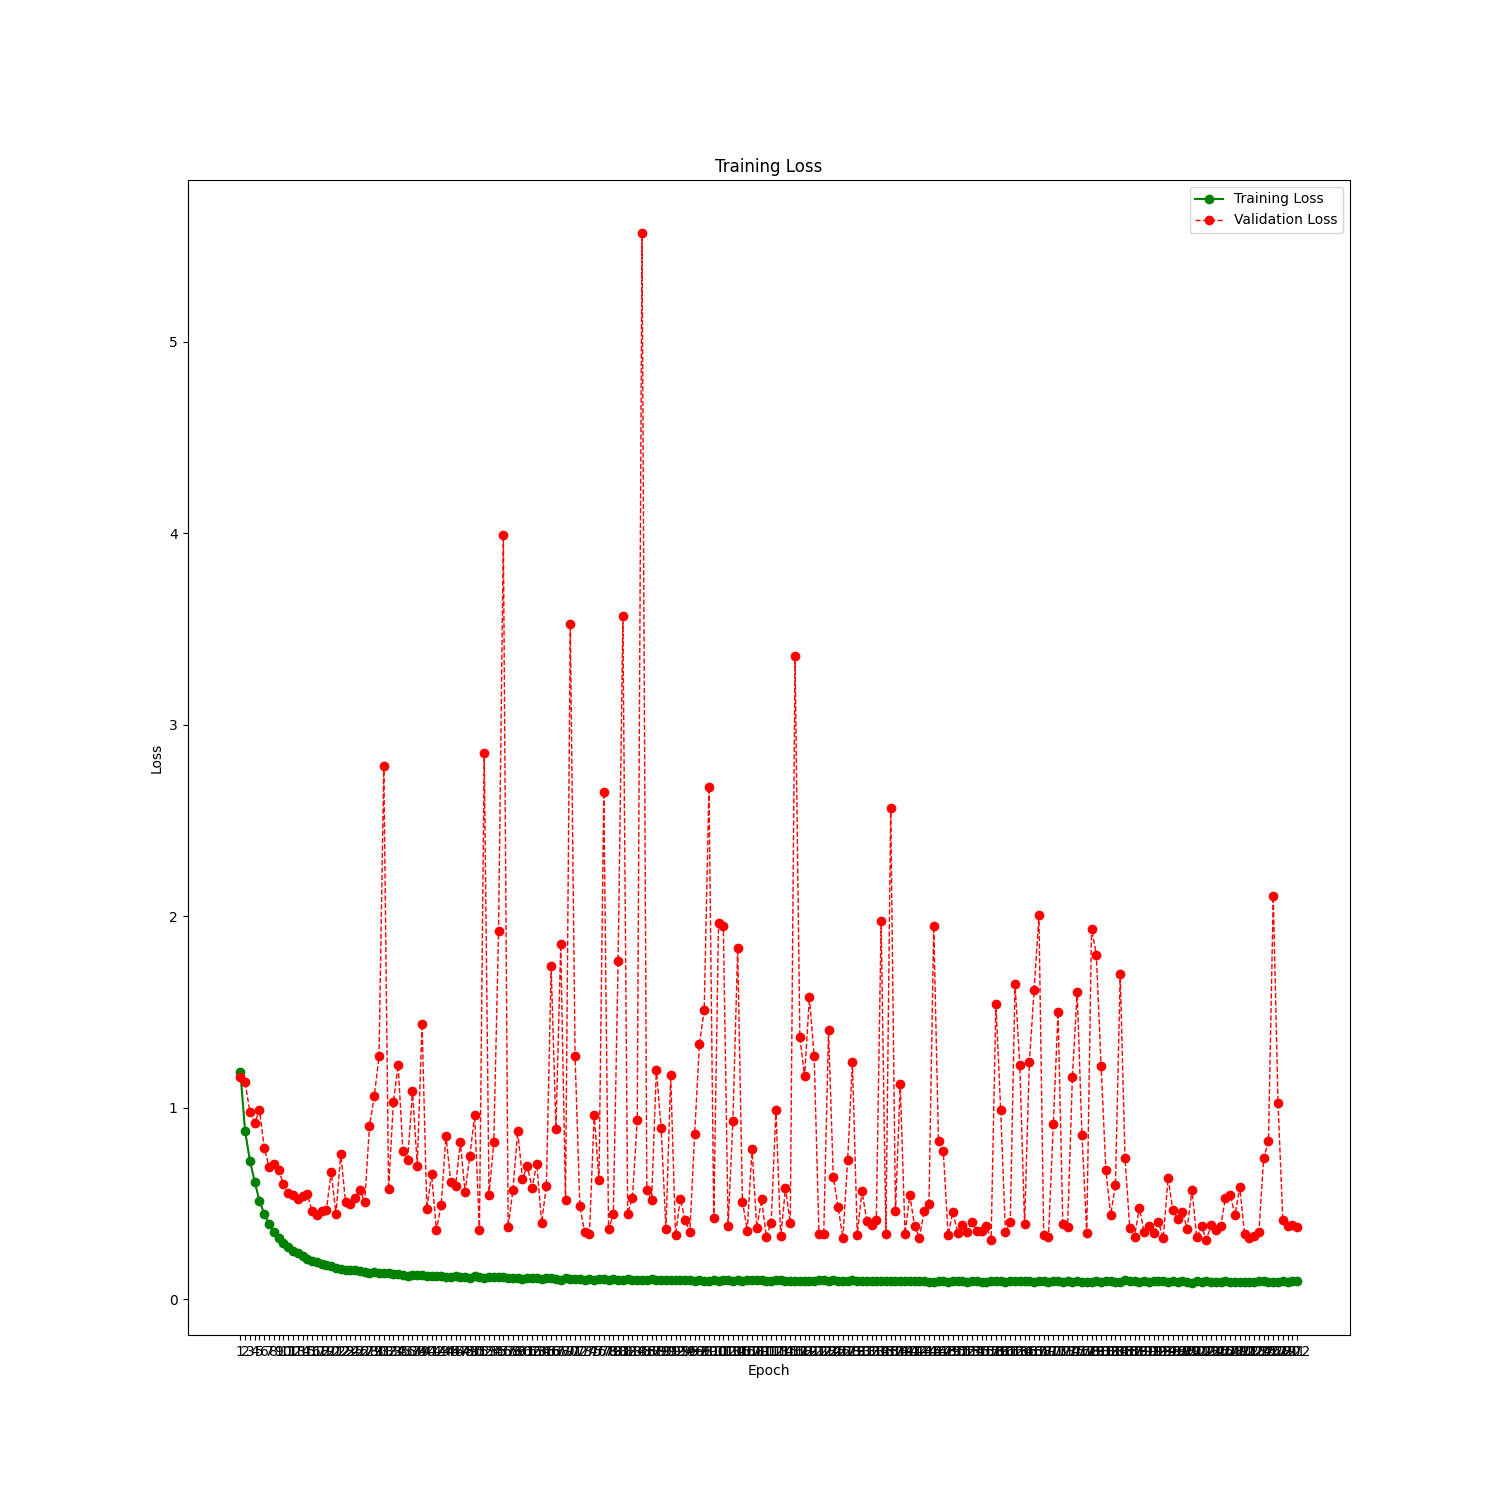
\includegraphics[width=8.5cm]{images/progress_epoch_1_222.png}
    \caption{Training Progress from Epochs 1 - 222}
    \label{fig:epoch1}
\end{figure}

\subsubsection{Evaluation} \label{sec:eval}
As with other natural language processing applications, model evaluation becomes difficult when considering that a single input can be translated into many different correct sequences. For \LaTeX\, possible translations increase dramatically due to optional formatting tokens, e.g. \verb|x_i| vs. \verb|x_{i}| vs. \verb|{x}_i|. This is why CROHME evaluates using the symLG format rather than a \LaTeX\ sequence \cite{CROHME}. For more general applications, evaluation paradigms such as BLEU account for other translation possibilities \cite{BLEU}. 

As of the writing of this paper, the tools provided by CROHME to translate \LaTeX\ to symLG and thus evaluate a score are unavailable. As an alternative, this paper evaluates the VTex model using an approximation of the expression recognition rate (ExpRate). Specifically, the Levenshtein distance between the output and ground truth sequences is calculated, providing the number of transformations needed to convert the output to the ground truth. Table \ref{table:testresults} shows test accuracy from the 2016 and 2019 CROHME datasets for different margins of error. Only approximately 20-24\% of results had no errors at all, but once a margin of error of 1 is taken into account, the effective accuracy jumps to 35-40\%. 

The beam search algorithm performs better in the $\leq$5 and $\leq$10 error metrics, but greedy performs better in the 0-1 error metrics. In theory, beam search outperforms greedy in longer sequences, as beam search gives the decoder more chances to recover from an incorrect prior prediction. We believe that the increase in performance in the $\leq$5 and $\leq$10 error metrics is due to this property as test sequences falling into this category are likely to be longer. However, we are unsure why greedy performs better in the 0-1 error metrics. It is possible that the beam search algorithm misleads the decoder into diverging from the correct path, particularly with larger beam sizes.

Unfortunately, our model did not perform well compared to BTTR. BTTR adds several additional features VTex does not, including bidirectional training \cite{ZhaoBTTR2021}. In addition, BTTR is built on the PyTorch Lightning framework, which may provide improvements in training.

\begin{table}
\centering
    \begin{tabular}{|c | c | c | c |} 
     \hline
     Model & ExpRate & 2016 & 2019 \\
     \hline\hline
     \multirow{4}{4em}{VTex (beam search)} & 0 error & 20.65\% & 24.14\% \\
     & $\leq$1 error & 34.69\% & 39.77\% \\
     & $\leq$5 error & 64.80\% & 72.64\% \\
     & $\leq$10 error & 84.84\% & 90.46\% \\
     \hline
     \multirow{4}{4em}{VTex (greedy)} & 0 error & 21.67\% & 24.60\% \\
     & $\leq$1 error & 35.40\% & 39.31\% \\
     & $\leq$5 error & 62.97\% & 70.80\% \\
     & $\leq$10 error & 80.47\% & 87.36\% \\
     \hline
     \multirow{2}{4em}{BTTR} & 0 error & 52.31\% & 52.96\% \\
     & $\leq$1 error & 63.90\% & 65.97\% \\
     \hline
    \end{tabular}
\caption{Test Result Accuracy for 2016 and 2019 CROHME Datasets}
\label{table:testresults}
\end{table}
